\usetikzlibrary{lindenmayersystems}
\pgfdeclarelindenmayersystem{cayley}{
  \rule{F -> F [ R [F] [+F] [-F] ]}
  \symbol{R}{
    \pgflsystemstep=0.5\pgflsystemstep
  } 
}

\begin{figure}[ht]
    \centering
    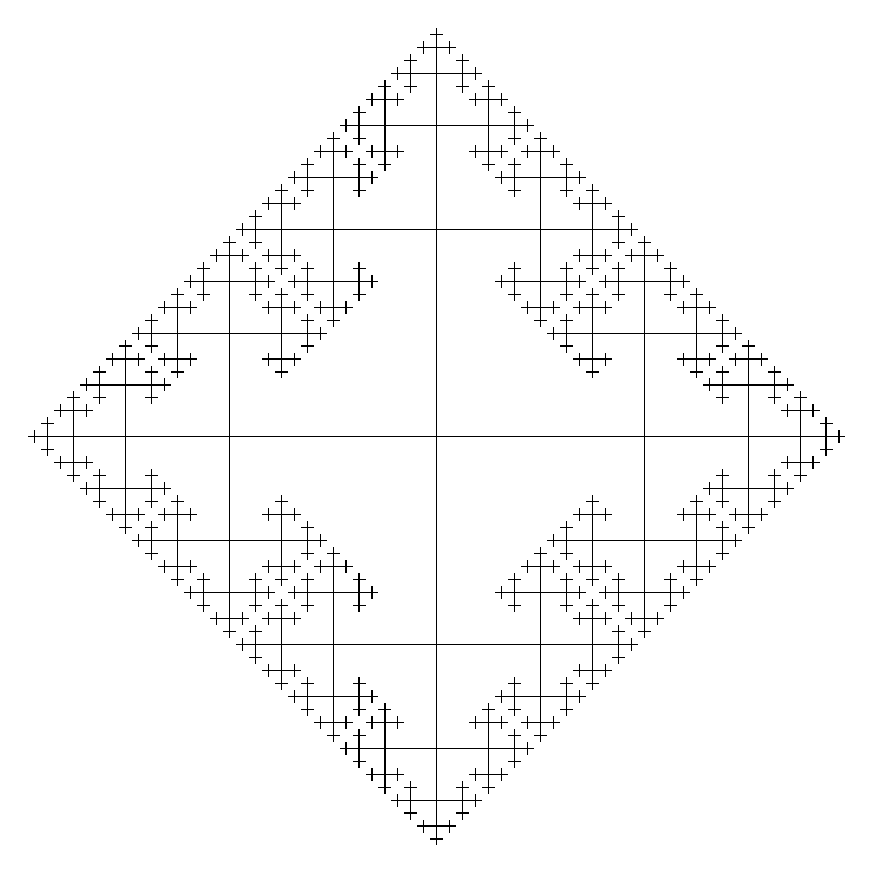
\begin{tikzpicture}
    \draw l-system [l-system={cayley, axiom=[F] [+F] [-F] [++F], step=75, order=5}];
    \end{tikzpicture}
    \caption{Representação de $Cay(F_2, \{a^{\pm 1}, b^{\pm 1}\})$, um fractal, de infinitas pontas.}
    \label{figure:cay(ab)}
\end{figure}